% ME3050 -  Dynamics Modeling and Controls - Tennessee Technological University
% Tristan Hill - Spring 2020 - Summer 2020 - Spring 2022
% Dynamics Modeling and Controls
% Lecture Module - Newtons Approach  - Topic 3 - Newton's Three Laws  
% Document settings

%\documentclass{beamer}                  % for presentation ?
\documentclass[handout]{beamer}  % for handout ?

\usepackage{../dmc_lectures} % .sty in parent folder

\newcommand{\MNUM}{3\hspace{2mm}} % Module number
\newcommand{\TNUM}{3\hspace{2mm}} % Topic number 
\newcommand{\moduletitle}{Newton's Approach }
\newcommand{\topictitle}{The Velocity Model } 

\newcommand{\sectiontitleI}{Example Problem - Quadcoptor Model}
\newcommand{\sectiontitleII}{Mathematical Modeling}
\newcommand{\sectiontitleIII}{Newton's Second Law Approach}
\newcommand{\sectiontitleIV}{Derived Equations of Motion}

\author{ME3050 - Dynamic Modeling and Controls}
\title{Lecture Module - \moduletitle}
\date{Mechanical Engineering\vspc Tennessee Technological University}

\begin{document}
	
	\lstset{language=MATLAB,basicstyle=\ttfamily\small,showstringspaces=false}
	
	\frame{\titlepage \center\begin{framed}\Large \textbf{Topic \TNUM - \topictitle}\end{framed} \vspace{5mm}}
	
	% Section 0 - Outline
	\frame{
		
		\large \textbf{Topic \TNUM - \topictitle} \vspace{3mm}\\
		
		\begin{itemize}
			
			\item \sectiontitleI    \vspc % Section I
			\item \sectiontitleII 	\vspc % Section II
			\item \sectiontitleIII 	\vspc %Section III
			\item \sectiontitleIV 	\vspc %Section IV
			%\item \sectiontitleV 	\vspc %Section V
			
		\end{itemize}
		
	}

% Section I:
\section{\sectiontitleI}

\frame{
\frametitle{\sectiontitleI}

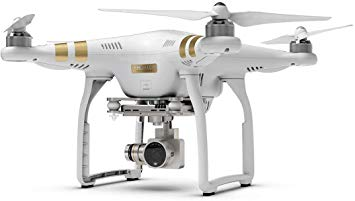
\includegraphics[scale=0.35]{dji_phantom.jpg}
\begin{framed}
\underline{Problem Statement} -  \vspccc

\end{framed}

{\tiny Image: source needed}
}

% Section II:
\section{\sectiontitleII}

\frame{
\frametitle{\sectiontitleII}

First, consider the physical problem and list all simplifying assumptions necessary or desired. In general, the designed should start simple and add complexity incrementally. \vspc

\underline{Quadcopter Model Assumptions:}

\begin{enumerate}
\item
\item
\item
\end{enumerate}

}

% Section III:
\section{\sectiontitleIII}

\frame{
\frametitle{\sectiontitleIII}

\textbf{ \Large \underline{Newton's Second Law Approach} }\\
\begin{enumerate}
\item \vspace{3mm}
\item \vspace{3mm}
\item \vspace{3mm}
\item \vspace{3mm}
\item \vspace{3mm}
\end{enumerate}

}

\frame{
\frametitle{\sectiontitleIII \hspace{1mm} - Steps 1,2 and 3}


}
	
\frame{
\frametitle{\sectiontitleIII \hspace{1mm} - Steps 4,5}


\begin{tabular}{ccc}
Translation:&$\Sigma {\bf F}=m{\bf a}$&$ \Sigma F_x=ma_x$\\
&&$\Sigma F_y=ma_y$\\
&&$\Sigma F_z=ma_z$ \\
&&\\
Rotation: &$\Sigma {\bf M}=I_o{\bf \alpha}$&$\Sigma M_o=I_o\alpha_z$\\
\end{tabular}

}	
	
% Section IV:
\section{\sectiontitleIV}

\frame{
\frametitle{\sectiontitleIV}



}	
	
\end{document}





